\documentclass[runningheads]{llncs}
%
\usepackage{graphicx}

\begin{document}
%
    \title{AAQC - Autonomous air quality control}

%\author{Smart Cities and Internet of Things - Group 16: \\
%Tobias Haller (\texttt{3132111}) \email{st141219@stud.uni-stuttgart.de}\\
%Jonas Hofer (\texttt{XXXXXXX}) \email{st173462@stud.uni-stuttgart.de} \\
%Christian M\"uller (\texttt{3132108}) \email{st140956@stud.uni-stuttgart.de}}

    \author{Group 16 - Tobias Haller \and Jonas Hofer \and Christian M\"uller}

    \institute{Service Computing Department, IAAS, University of Stuttgart}

%
    \maketitle              % typeset the header of the contribution
%
%\begin{abstract}
%    The abstract should briefly summarize the contents of the report in
%    150--250 words. 
%    
%    \keywords{First keyword  \and Second keyword \and Another keyword.}
%\end{abstract}


    \section{System Introduction}
Increasing the well-being of people is an important topic of research. Especially for office spaces, when companies want to increase the efficiency of their employees. In general, with good air in terms of proper temperature, humidity and air purity, people feel more comfortable and can be considered healthier and more productive than with poor quality air. \\
Another application could be retail stores where customers stay longer if they feel more comfortable, which could lead to higher revenue for the retail business. Of course, businesses also face great competition from online retailers and other stores where air monitoring and customer comfort could be the difference or advantage. \\
Since we are participating in the lecture "Smart Cities and IoT", we want to gain practical experience in addition to the theoretical basics taught in the lecture. In our project, we will consider a single office space that controls heating, air conditioning, ventilation and air purifier according to several sensor measurements, thus monitoring the air quality. Since this example can be easily scaled up to large enterprises with many office rooms, we can easily test the system using a single room as a POC. Moreover, we only need to change some thresholds to extend the scope to retail stores or other buildings. Based on this basic problem definition and the main scope of our work, in the following we will specify our use cases and requirements for a system that should automate such tasks as well as some additional tasks for a user.


    % TRASH -----------------------------------------------------------------------------------------------------
    % Increasing people's efficiency and comfort is an important topic of research.
    % Making everyday life more comfortable and easier is a predominant aspect of development related to smart buildings and especially smart homes.
    % Therefore, it is not surprising that companies offering solutions for smart cities and smart home devices have significant market growth.
%
    % Since we are participating in the lecture "Smart Cities and IoT" we want to gain practical experience in addition to the theoretical fundamentals taught by the lecture.
    % Since Smart Cities are just a bigger model or a further development of a smart home system, we will consider a smart home system as our project.
%
    % Let's assume we live in an appartement with e.g. a kitchen, a bathroom, a living room and a bedroom.
    % Since we have a huge music affinity we want to listen the whole day to music while moving in our appartement.
    % Without any smart home functionality we would have to turn on the speakers in the room we are currently in or turn it off once again when leaving.
    % Additionally, of course we would have to connect our smartphone to some speaker first and play our favorite music.
    % Once we got established the connection and the music is playing we would have to regulate the volume of the music according to many factors such as noise in the room.
%
    % In the following based on this basic problem definition and main scope of our work we want to specify our use cases and requirements for a smart home system which aims to automate such tasks as well as some additional ones for a user.


    \section{System Analysis}
    There are some core requirements and functionalities a user wants from this autonomous system.
    Given the described scenario we want to improve the situation of users by providing an autonomous way to control and adjust the air quality of a given room.
    In addition we want to improve comfort of users by also regulating temperature or humidity of a given room based on environmental factors.
    Another part of our system is to identify human presence or out of office time and adjust the functionality of the system accordingly.

    The core system functions will be separated into both functional and non-functional requirements according to ISO 25010.
    All requirements will be priorized by - - / - / 0 / + and ++, where all requirements with + or ++ are considered to be mandatory for our project.
    All other requirements are considered desirable or optional.

    \subsection{Functional Requirements}

    \begin{description}
        \item[Name] FA-1
        \item[Title] Autonomous temperature regulation
        \item[Description] The system should be able to regulate the temperature of the room based on system information and human presence
        \item[Dependencies] FA-8 FA-10
        \item[Priority] +
    \end{description}

    \begin{description}
        \item[Name] FA-2
        \item[Title] Autonomous humidity regulation
        \item[Description] The system should be able to regulate the humidity of the room based on system information and human presence
        \item[Dependencies] FA-9 FA-10
        \item[Priority] +
    \end{description}

    \begin{description}
        \item[Name] FA-3
        \item[Title] Autonomous air quality regulation
        \item[Description] The system should be able to regulate the air quiality of the room based on system information and human presence. Particle count (Particulate matter) and $CO_2$ concentration are the basis for measuring the air quality.
        \item[Dependencies] FA-6 FA-7 FA-10
        \item[Priority] ++
    \end{description}

    \begin{description}
        \item[Name] FA-4
        \item[Title] Night regulation
        \item[Description] The System should reduce its functionality to a minimum during night time.
        \item[Dependencies] FA-1 FA-2 FA-3
        \item[Priority] 0
    \end{description}

    \begin{description}
        \item[Name] FA-5
        \item[Title] Display system activity to User
        \item[Description] The System should be able to show its activity and monitoring information to the user
        \item[Dependencies] Everything else
        \item[Priority] - -
    \end{description}

    \begin{description}
        \item[Name] FA-6
        \item[Title] Recognize stale air
        \item[Description] The System should be able to recognize when the air has gone stale. This is based on the $CO_2$ concentration indoors.
        \item[Dependencies] None
        \item[Priority] ++
    \end{description}

    \begin{description}
        \item[Name] FA-7
        \item[Title] Recognize increased particulate matter concentration
        \item[Description] The System should be able to recognize when the air contains an increased concentration of particulate matter.
        \item[Dependencies] None
        \item[Priority] ++
    \end{description}

    \begin{description}
        \item[Name] FA-8
        \item[Title] Monitor indoor and outdoor temperature
        \item[Description] The System should be able to recognize the temperature indoors and outdoors of its operating location.
        \item[Dependencies] None
        \item[Priority] ++
    \end{description}

    \begin{description}
        \item[Name] FA-9
        \item[Title] Monitor indoor and outdoor humidity
        \item[Description] The System should be able to recognize the humidity indoors and outdoors of its operating location.
        \item[Dependencies] None
        \item[Priority] ++
    \end{description}

    \begin{description}
        \item[Name] FA-10
        \item[Title] Detect human presence
        \item[Description] The System should be able to detect human presence indoors.
        \item[Dependencies] None
        \item[Priority] -
    \end{description}

    \subsection{Non-functional Requirements}

    \begin{description}
        \item[ID] NFA-1
        \item[Title] Realworld application
        \item[Description] The system should be able to be easily transformed to a real world running smart home system.
        \item[Dependencies] None
        \item[Priority] -
    \end{description}

    \begin{description}
        \item[ID] NFA-2
        \item[Title] Automation with minimal user intervention
        \item[Description] The system should utilze AI-planning in order to automate its autonomous functionalities with minimal user intervention.
        \item[Dependencies] None
        \item[Priority] ++
    \end{description}

    \begin{description}
        \item[ID] NFA-3
        \item[Title] Loosely coupled system
        \item[Description] The system should be loosely coupled regarding its communication between devices.
        \item[Dependencies] None
        \item[Priority] ++
    \end{description}


    \section{System Architecture Design}

    In the following we will specify our main components that execute our main functionalities. All components are separated into the following Layers according to ISO/OSI Model.

    \begin{figure}
        \centering
        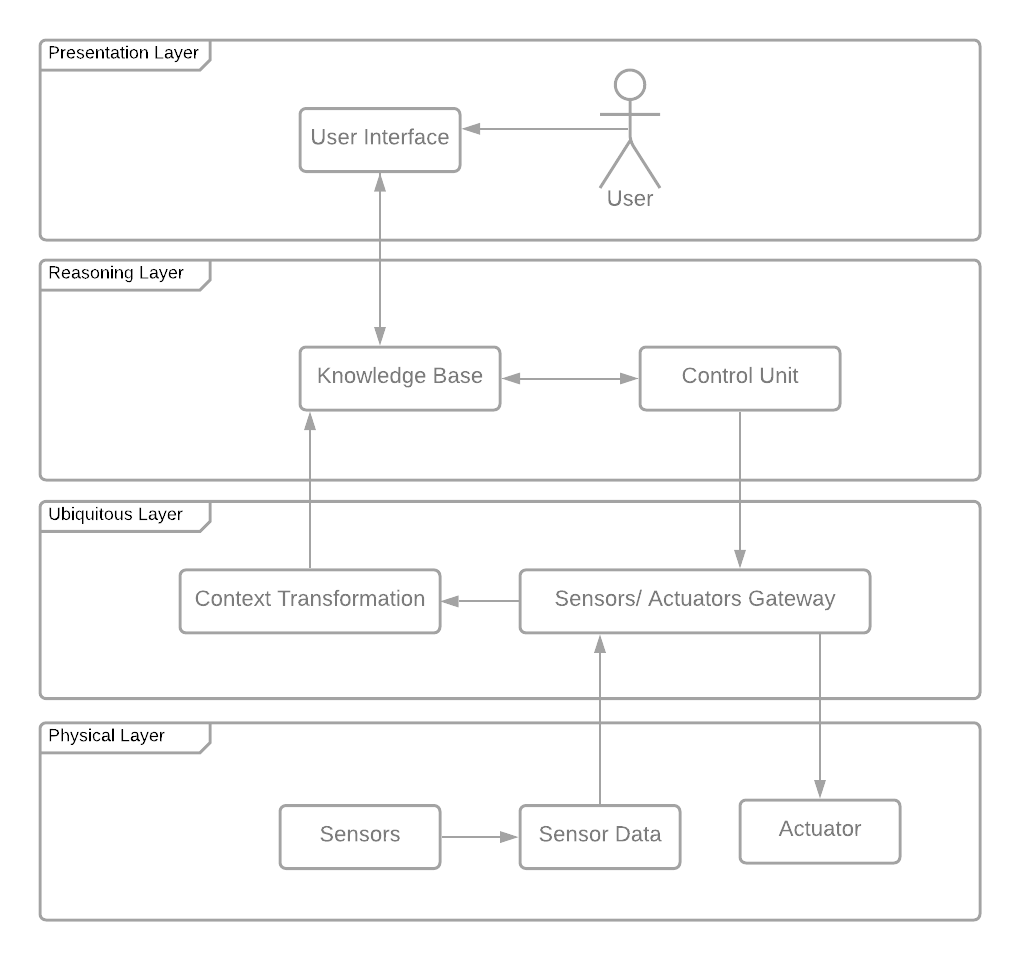
\includegraphics[width=\linewidth]{img/system-design.png}
        \caption{The system design illustrated as a diagram}
        \label{fig:system-design}
    \end{figure}

    \subsection{Presentation Layer}
    The Presentation Layer consists of the User Interface and the User itself. The (human) User interacts with our system via the User Interface which is a GUI. The user can monitor the system as described in functional requirement FA-5.

    \subsection{Reasoning Layer}
    The reasoning layer consists of the knowledge base and the control unit. The knowledge base stores all the sensor data that is generated and stores information about the individual room with the state of all the actuators. It receives all its data from the Context Transformation component in the Ubiquitous Layer. The Control Unit interacts closely with the Knowledge Base, as it receives a notification as soon as new sensor data is stored in the Knowledge Base. Based on all the data, the Control Unit decides based on AI-planning what actions it should take next. As soon as it has reached a conclusion and formulated a plan, it communicates this plan with the Sensors/Actuators gateway in the Ubiquitous Layer.

    \subsection{Ubiquitous Layer}
    The main component of the ubiquitous layer is the sensor/actuator gateway which communicates between the physical layer devices and the components of the reasoning layer. It will process commands from the control unit of the reasoning layer directly in order to relay commands to the actuators of the system. Sensor data however will be given to the Context Transformation component which has the job to take this raw data and transform it to a more precise and informative format which will then be communicated with the knowledge base of the reasoning layer.

    \subsection{Physcial Layer}
    There are two main components of the physical layer. Firstly the sensor which produces sensor data that will be sent to the gateway. Sensors will be used to satisfy functional requirements such as FA-8 and others. Secondly actuators will get instructions from the gateway and execute upon these as is described in the functional requirements.

    \section{System Implementation}

    \subsection{Architecture}

    \subsection{Core}
    The application core is written using the C\# programming language and consists of three different parts. Firstly The AI Planning which will be further elaborated in (TODO). Additionally, a messaging endpoint component which has the job to receive incoming messages from the MQTT broker as well as send outgoing messages to this MQTT broker. This communication will be explained in detail in (TODO). Furthermore, the application core has an HTTP API endpoint from which the User Interface, which is topic of (TODO), can get user relevant information about the sensor measurements and current state of the systems actuators. 

    The communication inside the Core differs for the communication between the messaging endpoint and the AI Planning and the communication between the AI Planning and the HTTP API. 
    The AI Planning component and HTTP API do not communicate directly with each other. Instead the AI Planning component saves some of the information about its current state, namely sensor data and actuator states, inside an external application state store. In our implementation this is realized using a Redis cache, but this could also be substituted with a regular relational database such as any SQL database, given an implementation has been provided based on our given interface. The HTTP API can then look up the saved information it needs and send it to the requester. 
    The communication between the messaging endpoint and the AI Planning is more tightly coupled in contrast. These two components communicate directly through application intern function calls. On one hand the AI Planning does this when it has found changes in the current actuator state after it has finished one run of its planning routine. On the other hand the messaging endpoint does this periodically, so the AI Planning routine is not executed every time a new sensor measurement is sent to the MQTT broker. 

    \subsection{AI Planning}
    The AI Planning routine is implemented using a mix between an external AI Planner and internal programming logic. It is the central part of the application core and therefore also implemented using C\#. 

    The planning routine is initialized with the latest measurement of all sensors of the system in the so-called sensor context. All sensor measurements of this sensor context are uniquely identifiable for the AI Planning in order to know which physical location they come from. 

    \subsubsection{Sensor context evaluation}
    In a first step the AI Planning component evaluates this sensor context. There are different evaluation steps depending on the type of a sensor. The system has four different types of sensors which are the following:
    \begin{itemize}
        \item Temperature
        \item Humidity
        \item Particulate matter
        \item CO2
    \end{itemize}

    Each sensor measure will be evaluated in relation to certain threshold values. Depending on the sensor type there are is either a threshold above or below which we want to take action or an acceptable value range above or below which we want to take action. For example the evaluation of a temperature measure of $30^\circ$C indoors will be considered above a pre-defined temperature threshold for indoor rooms and therefore be too high. After the application finishes this sensor context evaluation it will have a sensor state in which all relations with the given thresholds of this sensor have been saved. 

    \subsubsection{PDDL domain}
    In this implementation we want a PDDL domain which is able to generate us any plan, which can be parsed and if necessary filtered or transformed to some extent, that lets us know the new state of our actuators, precisely if any of them are activated of deactivated. For this initialization, we can only use the previously evaluated sensor state as well as the current actuator state that we have saved inside the application state store. 

    \paragraph{Types}
    The general Idea behind the Types is that we have both actuators and sensors at the core. Actuators are modelled as a 'device' type and sensors as a 'sensor' type. The sensors are then separated into which type of sensor they are, e.g. temperature, humidity, air purity or co2. Functionally, this would be sufficient to model the domain, however to improve readability and therefore make changes to the domain easier there are more types. Each Actuator, namely the ventilation, heater, air conditioner and air purifier have a type of their own. Additionally, Each sensor type has a type of their own that also has where this sensor is located, e.g. 'temperature-in' which is of type temperature.

    \paragraph{Predicates}
    Most predicated of this domain will describe the sensor relation towards our given value or value range thresholds, as explained in (TODO). This relation was already saved inside the sensor state and will be somewhat reflected in the predicated that were chosen to describe our PDDL domain. The following predicates currently exist in our domain:
    \begin{itemize}
        \item \textbf{(on ?d - device)}: This predicate is used to determine which actuator, and therefore the potential device which it controls, is currently on. If this predicate is true the actuator is activated and if it is false the actuator is deactivated. 
        \item \textbf{(temperature-high ?t - temperature)}: This predicate together with the temperature-low predicate shows if a given temperature from a sensor is deemed not normal or acceptable. There need to be two predicated designated to modelling a threshold relation if the accepted value is a range. In this case, if the temperature-high predicate is true the temperature is too high, otherwise if it is false the temperature can be either normal or too low. Therefore, if both temperature-high is false and temperature-low is false, we know that the temperature for a given sensor is normal. 
        \item \textbf{(temperature-low ?t - temperature)}: As mentioned, this predicate together with the temperature- high predicate shows if a given temperature from a sensor is seemed normal or acceptable. If this predicate is true the temperature is too low and if it is false the temperature is either normal or too high. 
        \item \textbf{(humidity-high ?h - humidity)}: Unlike the temperature predicated where we needed multiple ones to model the sensor state, for humidity we are only interested if the humidity is too high. Therefore, if this predicate is true the humidity is too high otherwise if it is false the humidity is deemed acceptable. 
        \item \textbf{(air-purity-bad ?a - air-purity)}: This predicate is used to determine the air purity, namely if there is too much particulate matter in the air. If this predicate is true we deem the air purity bad and if it is false the air purity is deemed acceptable.
        \item \textbf{(co2-level-emergency ?c - co2-level)}: This predicate indicates if the co2 level, in this case inside a given room, is either too high in which case this predicate is true or it is not too high and deemed acceptable in which case this predicate is false. This is a very problematic case and the system has to react more extremely to this than for other cases. 
    \end{itemize}

    \paragraph{Actions}
    The actions of our PDDL domain are exclusively related to activating or deactivating the actuators. There are these following actions: 
    \begin{itemize}
        \item activateVentilation
        \item deactivateVentilation
        \item activateHeater
        \item deactivateHeater
        \item activateAirConditioner
        \item deactivateAirConditioner
        \item activateAirPurifier
        \item deactivateAirPurifier
    \end{itemize}

    \subsubsection{Parsing sensor and actuator state to PDDL problem}
    The PDDL problem we want to generate depends on both the sensor state, which we evaluated previously, and the actuator state, which we received from the application state store. Additionally, the PDDL domain is the basis for any PDDL problem we want to generate. 

    The objects of any problem we generate is identical. Here we create an object for any actuator as well as all sensors of our system. For our problem, we need objects of the following types: 
    \begin{itemize}
        \item ventilation
        \item heater
        \item air-conditioner
        \item air-purifier
        \item temperature-in
        \item temperature-out
        \item humidity-out
        \item air-purity-in
        \item air-purity-out
        \item co2-level-in
    \end{itemize}

    The initial states of a PDDL problem is the most interesting part, since these depend on the sensor measurements and the current actuator state. Actuator initial states are based on if they are active or not. 
    For active actuators, each will have an 'on' predicate added to the init of the problem. Due to the close world assumption of PDDL inactive actuators will not be part of the problem init section. 
    The sensor state will also be parsed to init predicates of the PDDL problem. Here we will add the predicates as is described in (TODO) to the problem init. Since we only have unwanted behavior as sensor predicates if there are no sensor predicates, we know the system is in a state where we do not need to activate any actuators. This is also the case for the actuators, since the best case for our system is that all sensor measurements are acceptable and all actuators are deactivated. This fact already describes what goal our PDDL problem will have. Furthermore, if any problem we create has no initial states, we also know that no action has to be taken without consulting any external AI Planner at all. This is due to the fact that such an initial state would mean all actuators are deactivated and any sensor measures acceptable values.

    The goal of our problem is always the same. Find a plan for our current system, after which all actuators are deactivated and all sensor measurements inside the room our system runs for are acceptable. Precisely, we want the temperature to be neither too high nor too low, we do not want the air purity to be bad and there should not be too high of a co2 concentration inside the room. For our goal, the state of the outside sensors is irrelevant, since that is not something our system can change.

    \subsubsection{Create PDDL plan via external AI Planner}
    In order to create any plan, our application has to interact with some external AI Planner which can create such a plan based on the given PDDL domain and problem. In order to stay flexible regarding which external AI Planner wants to be used, we provide an interface which has to be implemented. This interface gets a PDDL problem and returns a list of steps the plan consist of. If this list is either empty or null, we know that we don't have to do anything and can conclude the current AI Planning routine. 

    For our implementation we used an online pddl solver (TODO footnote http://solver.planning.domains). Here we can just send an HTTP request with the domain and problem file and this planner will return a response with the plan and some other meta information. For this requesting, we used Flurl (TODO footnote).

    \subsubsection{Parse PDDL plan and execution}
    Due to the way our PDDL domain and the PDDL problem is modeled, a given plan can not be takes completely at face value. We need to filter the given plan somewhat to get which actuators we have to activate or deactivate.

    Since part of the goal of our problem is that all actuators are deactivated, a given plan will contain a step for activating as well as deactivating said actuator in the cases where in reality we only want to activate this actuator. This however can easily be filtered out by looking at which activation action have a paired deactivation step, since in practice we do not want to activate and deactivate an actuator in the same planning routine. This is not the case for deactivation, therefore, if there is only a deactivation step present in the plan we know that we really want to deactivate this actuator.

    This filtering and parsing step will result in a new actuator state like the one we initially used before going into the PDDL problem parsing. This actuator state will have all states of the system's actuators, namely if they are activated or deactivated. If this new actuator state is the same as the one we used going into the planning, we know that nothing has changed, and we can successfully finish the AI planning routine. If this is not the case, we will transform this information into the message format which the messaging endpoint wants and send such a message for each actuator for which we want to change its state. Finally, if there are changes in the actuator state, we will save the new actuator state inside the application state store, so it is up-to-date.

    \subsection{Communication}

    \subsection{Simulation}

    \subsection{User Interface}


% \section{Discussion and Conclusions}
% Here you can discuss some interesting points or limitations of your system and conclude the report.

%
% ---- Bibliography ----
%
%\bibliographystyle{splncs04}
%\bibliography{mybib}

%All links were last followed on \today.

\end{document}
